\subsection{Стохастическая чувствительность}

    Для аппроксимации вероятностного распределения случайных состояний вокруг детерминированных аттракторов (равновеися или циклов) можно использовать сетод функции стохастический чувствительности. Данный подход описан в работе Ряшко Л. Б. \cite{Ryashko}.

    На графике \ref{bifurcation_x_0_2_a_1_beta_chaos_fss} красными линиями изображена функция стохастической чувствительности. 

    \begin{figure}
        \centering
        \subfloat[Общий вид бифуркационной диаграммы с ФСЧ]{
            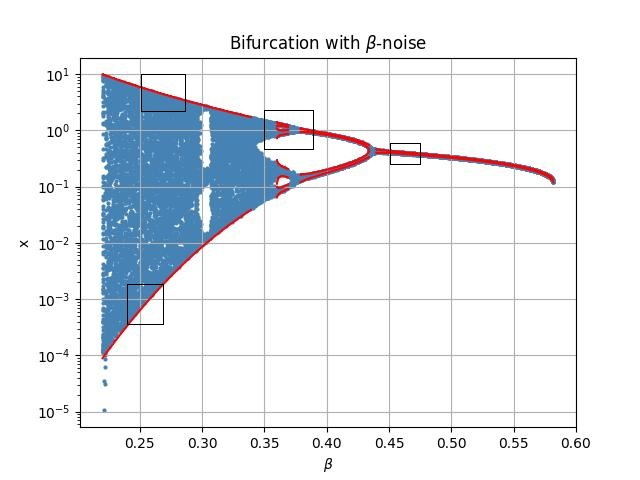
\includegraphics[width=0.7\textwidth]{stochastic/images/bifurcation_x_0_2_a_1_beta_noise_fss.jpg}
            \label{bifurcation_x_0_2_a_1_beta_chaos_fss}
        }

        \subfloat[ФСЧ для равновесия]{
            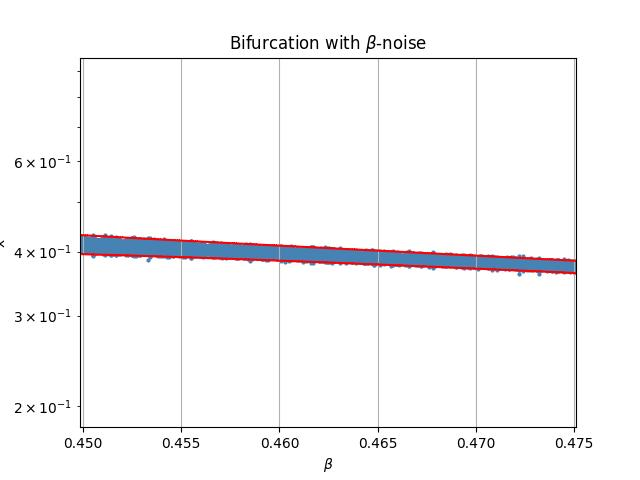
\includegraphics[width=0.5\textwidth]{stochastic/images/bifurcation_x_0_2_a_1_beta_noise_fss_segment_stable.jpg}
            \label{bifurcation_x_0_2_a_1_beta_chaos_fss_segment_stable}
        }  
        \subfloat[ФСЧ для 2-цикла]{
            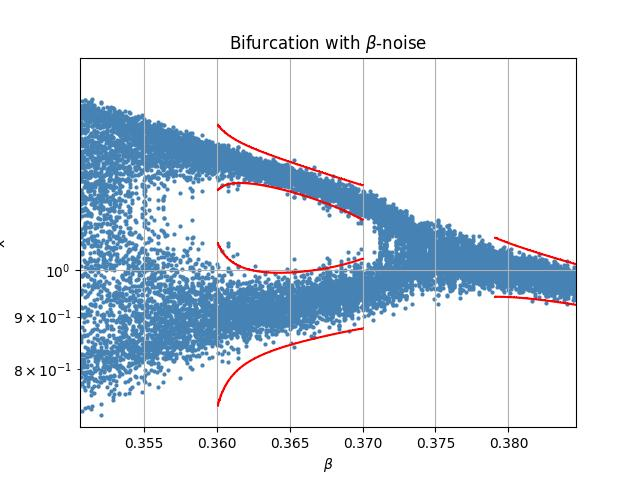
\includegraphics[width=0.5\textwidth]{stochastic/images/bifurcation_x_0_2_a_1_beta_noise_fss_segment_2_cycle.jpg}
            \label{bifurcation_x_0_2_a_1_beta_chaos_fss_segment_2_cycle}
        }
            
        \subfloat[ФСЧ для хаоса]{
            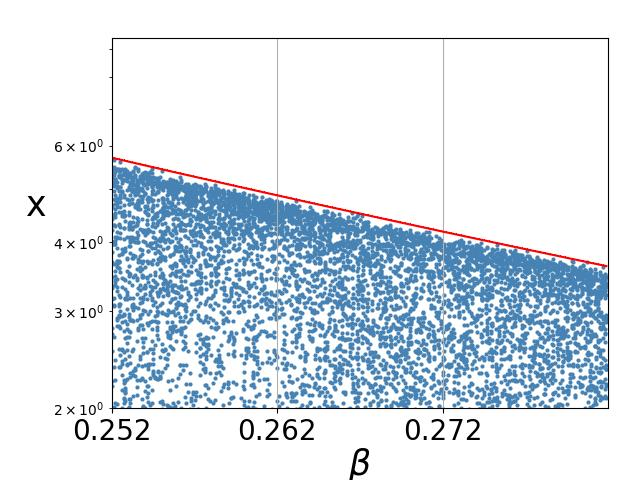
\includegraphics[width=0.5\textwidth]{stochastic/images/bifurcation_x_0_2_a_1_beta_noise_fss_segment_chaos_up.jpg}
            \label{bifurcation_x_0_2_a_1_beta_chaos_fss_segment_chaos_up}
        }
        \subfloat[ФСЧ для хаоса]{
            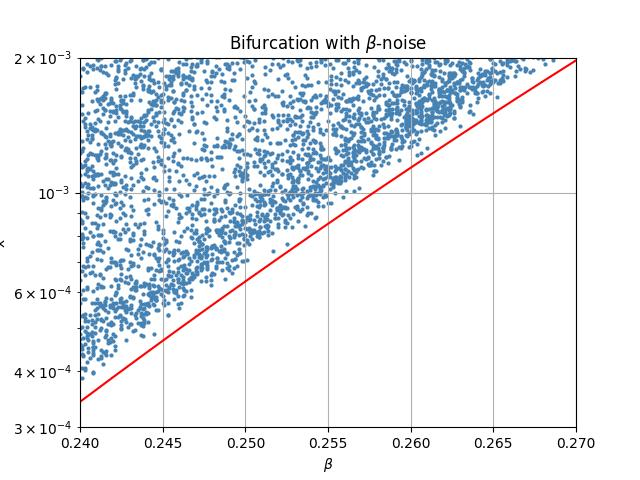
\includegraphics[width=0.5\textwidth]{stochastic/images/bifurcation_x_0_2_a_1_beta_noise_fss_segment_chaos_down.jpg}
            \label{bifurcation_x_0_2_a_1_beta_chaos_fss_segment_chaos_down}
        }
            
        \caption{Бифуркационная диаграмма с ФСЧ для модели \ref{beta_chaos}}
    \end{figure}

    Рассмотрим участок от \(\beta \approx 0.45\) до \(\beta \approx 0.48\), он изображен на рисунке \ref{bifurcation_x_0_2_a_1_beta_chaos_fss_segment_stable}. Мы видим, что значения графика бифуркации почти всегда находятся в коридоре, границами которого являются значения ФСЧ. Этот коридор строится по правилу трех сигм. Такой подход гарантирует, что почти все значения будут находиться в этом интервале, что собственно мы и наблюдаем.

    На участках с k-циклами и хаосом (рисунки \ref{bifurcation_x_0_2_a_1_beta_chaos_fss_segment_2_cycle}, \ref{bifurcation_x_0_2_a_1_beta_chaos_fss_segment_chaos_up} и \ref{bifurcation_x_0_2_a_1_beta_chaos_fss_segment_chaos_down}) будет наблюдаться аналогичная ситуация: значения лежат в коридоре, ограниченном значениями ФСЧ.
